\documentclass[12pt]{report}
\usepackage{listings}
\usepackage{amsmath}
\usepackage[pdftex]{graphicx}
\usepackage{fancyvrb}
\usepackage{chapterbib}
\usepackage{hyperref}
\usepackage{listings}
\usepackage{wrapfig}
\usepackage{subfig}
\usepackage{algorithm}
\usepackage{algorithmic}
\usepackage{esint}
\usepackage{amssymb}
\usepackage[usenames]{color}
\usepackage[toc,page,title,titletoc]{appendix}

\pdfcompresslevel=9
\DeclareGraphicsExtensions{{.png},{.pdf},{.jpg},{jpeg}}
\graphicspath{ {../figures/}}
\usepackage{color}
%__________________________________
% new commands for all sections
\newcommand{\comment}[1]{ \marginpar{{\scriptsize \color{red} #1 }}}
\newcommand{\red}[1]{\color{red} {#1} \color{black}}
\newcommand{\TT}[1]{\tt{#1}\normalfont}

% MPM & ICE
\newcommand{\tn}[1]{\mbox{\bf{#1}}}
\newcommand{\sig}{\mbox{\boldmath $\sigma \!\!$ \unboldmath}}
\newcommand{\bnabla} {\mbox {\boldmath $\nabla \!\!$ \unboldmath}}
\newcommand{\taubold} {\mbox{\boldmath $\tau \!\!$ \unboldmath}}
\newcommand{\f}{\ensuremath{f^{\theta}_r} }

\newcommand{\Texp}{\rm{exp}}
\newcommand{\Text}{\rm{ext}}
\newcommand{\Tint}{\rm{int}}
\newcommand{\Teq}{\rm{eq}}
\newcommand{\Delt}{\ensuremath{\Delta t}}
\newcommand{\Ep}{\ensuremath{\epsilon_p}}
\newcommand{\Epi}{\ensuremath{\varepsilon_{pi}}}
\newcommand{\Epdot}[1]{\ensuremath{\dot{\epsilon}_{p#1}}}
\newcommand{\erf}{\text{erf}}
\def\bfE{{\bf E}}
\newcommand{\BD}{\ensuremath{\boldsymbol{D}}}
\newcommand{\Half}{\ensuremath{\frac{1}{2}}}
\newcommand{\Bsig}{\ensuremath{\boldsymbol{\sigma}}}
\newcommand{\Bn}{\ensuremath{\boldsymbol{n}}}
\newcommand{\Bg}{\ensuremath{\boldsymbol{g}}}
\newcommand{\Bd}{\ensuremath{\boldsymbol{d}}}
\newcommand{\BF}{\ensuremath{\boldsymbol{F}}}
\newcommand{\Bs}{\ensuremath{\boldsymbol{s}}}
\newcommand{\Tr}{\ensuremath{\text{tr}}}
\newcommand{\Beta}{\ensuremath{\boldsymbol{\eta}}}
\newcommand{\Beq}{\begin{equation}}
\newcommand{\Bone}{\ensuremath{\boldsymbol{\mathit{1}}}}
\newcommand{\Bu}{\ensuremath{\mathbf{u}}}
\newcommand{\Deriv}[2]{\ensuremath{\cfrac{d#1}{d#2}}}
\newcommand{\Eeq}{\end{equation}}
\newcommand{\norm}[1]{\ensuremath{\left\lVert#1\right\rVert}}
\newcommand{\Partial}[2]{\ensuremath{\frac{\displaystyle\partial #1}{\displaystyle\partial #2}}}
\newcommand{\That}{\ensuremath{\widehat{T}}}
\newcommand{\Xidot}{\ensuremath{\dot{\xi}}}


\def\rmd{{\rm d}}
\def\rme{{\rm e}}
\def\rmf{{\rm f}}
\def\rmr{{\rm r}}
\def\rmR{{\rm R}}
\def\rms{{\rm s}}
\def\bfd{{\bf d}}
\def\bfE{{\bf E}}
\def\bfF{{\bf F}}
\def\bff{{\bf f}}
\def\bfg{{\bf g}}
\def\bfI{{\bf I}}
\def\bfj{{\bf j}}
\def\bfm{{\bf m}}
\def\bfr{{\bf r}}
\def\bfx{{\bf x}}
\def\bfu{{\bf u}}
\def\rmg{{\rm g}}
\def\bfa{{\bf a}}
\def\bfG{{\bf G}}
\def\bfv{{\bf v}}
\def\tdot{{\textstyle\cdot}}
%__________________________________
\setlength{\textwidth}{15.5cm}
\setlength{\textheight}{21.5cm}
\setlength{\parskip}{0cm}        % paragraph skip


\begin{document}


\title{Uintah User Guide}


\author{ Jim Guilkey, Todd Harman, Justin Luitjens, \\ John Schmidt, Jeremy Thornock, J. Davison de St. Germain, \\ Siddharth Shankar, Joseph Peterson, Carson Brownlee, Charles Reid}

\date{Version 1.4.1}

\maketitle

\tableofcontents

%\begin{abstract}
%
%\end{abstract}

\newpage

%%
%% INTRODUCTION
%%
\chapter{Overview of Uintah} \label{Sec:Overview} 
The Uintah Computational Framework (also referred to as Uintah or the UCF)
consists of a set of
software components and libraries that facilitate the solution of
Partial Differential Equations (PDEs) on Structured AMR (SAMR) grids
using hundreds to thousands of processors.

One of the challenges in designing a parallel, component-based
and multi-physics application is determining how to efficiently decompose
the problem domain. Components, by definition, make local
decisions. Yet parallel efficiency is only obtained through a globally
optimal domain decomposition and scheduling of computational
tasks. Typical techniques include allocating disjoint sets of
processing resources to each component, or defining a single domain
decomposition that is a compromise between the ideal load balance of
multiple components. However, neither of these techniques will achieve
maximum efficiency for complex multi-physics problems.

Uintah uses a non-traditional approach to achieving parallelism by
employing an abstract task graph representation to describe
computation and communication. The task graph (see
Figure~\ref{fig:TaskGraph}) is an explicit representation of the
computation and communication that occur in the coarse of a single
iteration of the simulation (typically a timestep or nonlinear solver
iteration). Uintah components delegate decisions about parallelism to
a scheduler component by using variable dependencies to describe
communication patterns and characterizing computational workloads to
facilitate a global resource optimization. The task graph
representation has a number of advantages, including efficient
fine-grained coupling of multi-physics components, flexible load
balancing mechanisms and a separation of application concerns from
parallelism concerns. However, it creates a challenge for scalability
which we overcome by creating an implicit definition of this graph and
representing it in a distributed fashion.

%\begin{figure}
%  \includegraphics[scale=1]{Taskgraph-diagram.png}
%  \caption{Example Task Graph}
%  \label{fig:TaskGraph}
%\end{figure}

The primary advantage of a component-based approach is that it
facilitates the separate development of simulation algorithms, models,
and infrastructure. Components of the simulation can evolve
independently. The component-based architecture allows pieces of the
system to be implemented in a rudimentary form at first and then
evolve as the technologies mature. Most importantly, Uintah allows the
aspects of parallelism (schedulers, load-balancers, parallel
input/output, and so forth) to evolve independently of the simulation
components. Furthermore, components enable replacement of computation
pieces without complex decision logic in the code itself.

Please see the Developers Guide for more information about the
internal architecture of Uintah.

\section{Using Uintah} \label{Sec:UCF}

Several executable programs have been developed using the Uintah
Computational Framework (UCF).  The primary code is named \tt sus
\normalfont, which stands for Standalone Uintah Simulation.  The code
was originally developed to solve a complex fluid structure problem
involving a container filled with an explosive enveloped in a fire.
The code models the fire and the subsequent heat transfer to the
container followed by the resultant container deformation and ultimate
rupture due to the ignition and burning of the explosive material all
running on thousands of processors requiring thousands of hours of
computer time and hundreds of gigabytes of data storage.  Although
Uintah was developed originally to solve this complicated
multi-physics problem, the general nature of the algorithms and the
framework have allowed researchers to use the code to investigate a
wide range of problems.  The framework is general purpose enough to
allow for the implementation of FIX ME

This code leverages the task based parallelism inherent in the UCF to
implement several time stepping algorithms for structural mechanics,
fluid dynamics, and fluid structure interactions.  What follows is a
description of using \tt sus \normalfont within the realm of structural mechanics,
fluid mechanics, and structure-fluid interactions.



%__________________________________
\subsection{Mechanics of Running sus}
 - Explain how to run on multiple processors\\
 - what do the different command line options mean\\
 - how to restart an uda\\

For single processor simulations, the \tt sus \normalfont excutable
(Standalone Uintah Simulation) is run from the command line prompt
like this:
\begin{Verbatim}[fontsize=\footnotesize]
  
  sus <input.ups>

\end{Verbatim}
where \tt input.ups \normalfont is an xml formatted input file.  The Uintah
software release contains numerous example input files located in the
src/StandAlone/inputs directory.

For multiprocessor runs, the user generally uses \tt mpirun \normalfont to launch
the code.  Depending on the environment, batch scheduler, launch
scripts, etc, \tt mpirun \normalfont may or may not be used.  However, in general,
something like the following is used:
\begin{Verbatim}[fontsize=\footnotesize]

  mpirun -np num_processors sus -mpi input.ups

\end{Verbatim}
\tt num\_processors \normalfont is the number of processors that will be used.  The
input file must contain a patch layout that has at least the same
number (or greater) of patches as processors specified by a number
following the -np option shown above.

In addition, the \tt -mpi \normalfont is optional but often times necessary if the mpi
environment is not automatically detected from within the sus
executable.
 
%__________________________________
\subsection{Time Related Variables} \label{Sec:TimeRelatedVariables}
Uintah components are time dependent codes.  As such, one of the first entries
in each input file describes the timestepping parameters.  An input file
segment is given below that encompasses all of the possible parameters.
Most are self-explanatory, and not all are required,
(e.g \tt <max\_Timestep>,
<max\_delt\_increase>, <end\_on\_max\_time\_exactly> \normalfont and
\tt <delt\_init> \normalfont are all optional).
\tt <timestep\_multiplier> \normalfont serves
as a CFL number, that is, a number, usually less than 1.0, that is used to
moderate the timestep automatically calculated by the individual components. 

\begin{Verbatim}[fontsize=\footnotesize]
<Time>
    <maxTime>            1.0         </maxTime>
    <initTime>           0.0         </initTime>
    <delt_min>           0.0         </delt_min>
    <delt_max>           1.0         </delt_max>
    <delt_init>          1.0e-9      </delt_init>
    <max_delt_increase>  2.0         </max_delt_increase>
    <timestep_multiplier>1.0         </timestep_multiplier>
    <max_Timestep>       100         </max_Timestep>
    <end_on_max_time_exactly>true    </end_on_max_time_exactly>
</Time>
\end{Verbatim}
%
%__________________________________
\subsection{Data Archiver} \label{Sec:DataArchiver}
- variable labels\\
- checkpointing \\
- different options for specifying the output frequency\\
%
%__________________________________
\subsection{Geometry objects} \label{Sec:GeometryObjects}
- different objects available and how to specify them\\
- what is res \\
- operators, union, difference\\
- example of combining several geom\_objects\\

%__________________________________
\subsection{Boundary conditions}
- describe how to have a jet in the floor of the domain.
%
%__________________________________
\subsection{Grid specification} \label{Sec:Grid}
Explain how a grid is specified and what these tags mean

\begin{Verbatim}[fontsize=\footnotesize]
<Level>
    <Box label="1">
       <lower>        [0,0,0]          </lower>
       <upper>        [5,5,5]          </upper>
       <extraCells>   [1,1,1]          </extraCells>
       <patches>      [1,1,1]          </patches>
    </Box>
    <spacing>         [0.5,0.5,0.5]    </spacing>
</Level>
 \end{Verbatim}
%
%__________________________________
\subsection{Adapative Mesh Refinement}
- need to discuss the input options for the different regridders.\\
- How is a cell flagged as needing to be refined
%
%__________________________________
\subsection{load Balancer}
- to be filled in

%__________________________________
\subsection{UDA}

\subsubsection{UDA Directory Structure}

The UDA is a file/directory structure used to save Uintah simulation
data.  For the most part, the user need not concern him or herself
with the UDA layout, but it is a good idea to have a general feeling
for how the data is stored on disk...

%\subsubsubsection{UDA Naming}

Every time a simulation (sus) is run, a new UDA is created.  Sus uses
the <filebase> tag in the simulation input
(FIXME: link to [[Documentation/UsersGuide Input\_Files|.ups]]) file to name the UDA
directory (appending a version number).  If an UDA of that name
already exists, the next version number is used.  Additionally, a
symbolic link named ``disks.uda'' (is updated to and) will point to
the newest version of this simulations UDA.  Eg:

disks.uda.000
disks.uda.001
disks.uda.001 <- disks.uda

%\subsubsubsection{UDA Files}

Each UDA consists of a number of top level files, a checkpoints
subdirectory, and subdirectories for each saved timestep.  These files
include:

- \tt.dat\normalfont files contain global information about the simulation
(each line in the .dat files contains: simulation\_time value).
- The \tt checkpoints\normalfont directory contains a limited number of time
step data subdirectories that contain a complete snapshot of the
simulation (allowing for the simulation to be restarted from that
time).
- \tt input.xml\normalfont contains the original problem specification (the
.ups file).
- \tt index.xml\normalfont contains information on the actual simulation run.
- \tt t0000 FIXME number sign\normalfont contains data saved for that specific time step.  The
data saved is specified in .ups file and may be a very limited subset
of the full simulation data.

Example UDA file list:

CenterOfMassPosition.dat
CenterOfMassVelocity.dat
KineticEnergy.dat
StrainEnergy.dat
TotalMass.dat
checkpoints
index.xml
input.xml
t00001
t00057

%\subsubsection{Known Issues} 

Occasionally, due (most likely) to file system issues on large
clusters, some of the files in the UDA have been found to be corrupted
or nonexistent.  (There is error checking in the code to try to
prevent this.  We believe that either the OS/File system is
incorreclty returning error codes, or, more likely, that the files are
corrupted (due to file system issues) after the simulation is done.

%\subsubsection{Restrarting} 

FIXME: discuss how to modify an input parameter before you restart an uda.

%__________________________________
\subsection{Visualization tools}
- VisIT\\
- manta?

%__________________________________
\subsection{Tools}
- puda, lineextract, timeextract, compare\_uda\\

%__________________________________
\subsubsection{plotting tools}
- plotStats\\
- plotRegridder \\
- plotCPU\_usage \\
- plotComponents

%__________________________________
\subsection{Code}
-explain the basic directory structure of src
\begin{Verbatim}[fontsize=\footnotesize]
|-- CCA
|-- Components
|   |-- Angio
|   |-- Arches
|   |-- DataArchiver
|   |-- Examples
|   |-- ICE
|   |-- LoadBalancers
|   |-- MPM
|   |-- MPMArches
|   |-- MPMICE
|   |-- Models
|   |-- OnTheFlyAnalysis
|   |-- Parent
|   |-- PatchCombiner
|   |-- ProblemSpecification
|   |-- Regridder
|   |-- Schedulers
|   |-- SimulationController
|   |-- Solvers
|   |-- SpatialOps
|   `-- SwitchingCriteria
|-- Ports
|-- Core
|-- R_Tester
|-- StandAlone
|-- Teem
|-- VisIt
|-- build_scripts
|-- include
|-- orderAccuracy
|-- scripts
|-- tau
|-- testprograms
`-- tools
\end{Verbatim}

%% LyX 1.6.2 created this file.  For more info, see http://www.lyx.org/.
%% Do not edit unless you really know what you are doing.
\documentclass[english]{article}
\usepackage[T1]{fontenc}
\usepackage[latin9]{inputenc}

\usepackage{babel}

\begin{document}

\section{Arches}


\subsection{Introduction}

The Arches component solves a low-mach formulation with a pressure
projection of the Navier-Stokes equations for turbulent, variable
density, reacting flows. Turbulent flow scales are modeled using a
Large Eddy Simulation (LES) approach. Chemistry is handled using chemistry
parameterization and closure models for subgrid scale mixing. Modes
of heat transfer include radiation. blah blah blah


\subsection{Theory - Algorithm Description}

The essential governing equations for the Arches component, written
in finite volume form, include the mass balance, momentum balance,
mixture fraction balance, and energy balance equations. Using a bold-face
symbol to represent a vector quantity, the equations are: 
\begin{enumerate}
\item The mass balance, \begin{equation}
\int_{V}\frac{\partial\rho}{\partial t}dV+\oint_{S}\rho\mathbf{u}\cdot d\mathbf{S}=0\;,\label{eqn:mass_balance}\end{equation}
 where $\rho$ is density and $\mathbf{u}$ is the velocity vector. 
\item The momentum balance, \begin{equation}
\int_{V}\frac{\partial\rho\mathbf{u}}{\partial t}dV+\oint_{S}\rho\mathbf{uu}\cdot d\mathbf{S}=\oint_{S}\tau\cdot d\mathbf{S}-\int_{V}\nabla pdV+\int_{V}\rho\mathbf{g}dV\;,\label{eqn:mom_balance}\end{equation}
 where $\tau$ is the deviatoric stress tensor defined as $\tau_{ij}=2\mu S_{ij}-\frac{2}{3}\mu\frac{\partial u_{k}}{\partial x_{k}}\delta_{ij}$,
the second isotropic term in $\tau_{ij}$ is absorbed into the pressure
projection for the current low-Mach scheme, and $S_{ij}=\frac{1}{2}\left(\frac{\partial u_{i}}{\partial x_{j}}+\frac{\partial u_{j}}{\partial x_{i}}\right)$.
Also in Equation \ref{eqn:mom_balance}, $\mathbf{g}$ is the gravitational
body force and $p$ is pressure. 
\item The mixture fraction balance, \begin{equation}
\int_{V}\frac{\partial\rho f}{\partial t}dV+\oint_{S}\rho\mathbf{u}f\cdot d\mathbf{S}=\oint_{S}D\nabla f\cdot d\mathbf{S}\;,\label{eqn:species_balance}\end{equation}
 where $f$ is the mixture fraction and a Fick's law form of the diffusion
term assuming equal diffusivities results in a single diffusion coefficient,
$D$. 
\item The thermal energy balance, \begin{equation}
\int_{V}\frac{\partial\rho h}{\partial t}dV+\oint_{S}\rho\mathbf{u}h\cdot d\mathbf{S}=\oint_{S}k\nabla h\cdot d\mathbf{S}-\oint_{S}q\cdot d\mathbf{S}\;,\label{eqn:heat_balance}\end{equation}
 where $h$ is the sum of the chemical plus sensible enthalpy, $q$
is the radiative flux, a Fourier's law form of the conduction term
is used with a diffusion coefficient, $k$, and the pressure term
is neglected. 
\end{enumerate}
These equations are solved in an LES context, meaning filters are
applied to the equations. Here, we use Favre filtering, defined as
\[
\overline{\phi}=\frac{\overline{\rho\phi}}{\overline{\rho}},\]
 to isolate the density in the filtered equations. The filtering operations
result in the classic turbulence closure problem and thus models are
required. The model options are for Arches are discussed below. 

The set of filtered equations are discretized in space and time and
solved on a staggered, finite volume mesh. The staggering scheme consists
of four offset grids. One grid stores the scalar quantities and the
remaining three grids store each component of the velocity vector.
The velocity components are situated so that the center of their control
volume is located on the face centers of the scalar grid in their
respective direction. 

The equations are solved in an explicit manner. 


\subsection{Uintah Specification}


\subsubsection{Basic Inputs}


\subsubsection{Turbulence}


\subsubsection{Properties}


\subsubsection{BoundaryConditions}


\subsubsection{Physical Constants}


\subsubsection{Solvers}


\subsection{Examples}


\subsection{References}
\end{document}


\section{ICE} \label{Sec:ICE}


\subsection{Introduction}
\red{
finite volume
first order tempral discretizatioon
all speed
with the option of explicit or semi-implicit }

\subsection{Theory - Algorithm Description}

\subsection{Uintah Specification}
%______________________________________________________________________
\subsubsection{Basic Inputs}
The ICE component is selected by specifying:
%
Each Uintah component is invoked using a single executable called
\it sus \normalfont, which chooses the type of simulation
to execute based on the \it SimulationComponent \normalfont tag in the
input file.  In the case of ICE simulations, this looks like:

\begin{Verbatim}[fontsize=\footnotesize]
 <SimulationComponent type="ice" />
\end{Verbatim}
%
near the top of the inputfile.  The system of units \bf{must}\normalfont be
to be consistent (mks, cgs) and the majority of input files will be in meter-kilogram-sec
system.

%______________________________________________________________________
\subsubsection{Physical Constants}

\begin{Verbatim}[fontsize=\footnotesize]
<PhysicalConstants>
   <gravity>            [0,0,0]   </gravity>
   <reference_pressure> 101325.0  </reference_pressure>
</PhysicalConstants>
\end{Verbatim}

%______________________________________________________________________
\subsubsection{Material Properties}
For each ICE material the thermodynamic and transport properties must be
specified, in addition to the initial conditions of the fluid inside of
each geom\_object.  Below is the an example of how to specify an invisid
ideal gas over square region with dimensions $6m X 6m X 6m$.  The initial
conditions of the gas in that region are $T=300, \rho=1.179, v_x=1,v_y=2,
v_z=3$ \big{(}Note, the pressure XML tag is not used as an initial condition
and is simply there to make the user aware of what the pressure would be at
that thermodynamic state.\big{)}
%
\begin{Verbatim}[fontsize=\footnotesize]
<MaterialProperties>
   <ICE>
     <material>
       <EOS type = "ideal_gas">                </EOS>
       <dynamic_viscosity>   0.0               </dynamic_viscosity>
       <thermal_conductivity>0.0               </thermal_conductivity>
       <specific_heat>      716.0              </specific_heat>
       <gamma>              1.4                </gamma>
       <geom_object>
           <box label="wholeDomain">
               <min>       [ 0.0, 0.0, 0.0 ]  </min>
               <max>       [ 6.0, 6.0, 6.0 ]  </max>
           </box>
           <res>                 [2,2,2]      </res>
           <velocity>      [1.,2.,3.]         </velocity>
           <density>       1.1792946927374306 </density>
           <pressure>      101325.0           </pressure>     
           <temperature>   300.0              </temperature>
       </geom_object>
     </material>
  </ICE>       
</MaterialProperties>
\end{Verbatim}
%______________________________________________________________________
\subsubsection{Equation of State}
Below is a list of the various equations of state, along with the user defined
constants, that are available.  The reader should consult the literature for
the theoretical development and applicability of the equations of state to
the problem being solved.
%
%
The most commonly used EOS is the ideal gas law
\begin{equation}
  p = (\gamma -1) c_v \rho T
\end{equation}
%
and is specified in the input file with:
%
\begin{Verbatim}[fontsize=\footnotesize]
<EOS type="ideal_gas"/>
\end{Verbatim}
%
The Thomsen Hartka EOS for cold liquid water (1-100 atm pressure range)
is specified with \cite{ref:Thomsen,ref:bejan}
%
\begin{Verbatim}[fontsize=\footnotesize]
<EOS type="Thomsen_Hartka_water">
  <a>  2.0e-7     </a>    <!-- (K/Pa)     -->    
  <b>  2.6        </b>    <!-- (J/kg K^2) -->
  <co> 4205.7     </co>   <!-- (J/Kg K)   -->
  <ko> 5.0e-10    </ko>   <!-- (1/Pa)     -->
  <To> 277.0      </To>   <!-- (K)        -->
  <L>  8.0e-6     </L>    <!-- (1/K^2)    -->
  <vo> 1.00008e-3 </vo>   <!-- (m^3/kg)   -->
</EOS>
\end{Verbatim}
% 
%
The input specification for the ``JWLC'', ``JWL++'' and ``Murnahan'' equations of state from \cite{ref:JWL} are: 
\begin{Verbatim}[fontsize=\footnotesize]
<EOS type = "JWLC">
  <A>   2.9867e11   </A>
  <B>   4.11706e9   </B>
  <C>   7.206147e8  </C>
  <R1>    4.95      </R1>
  <R2>    1.15      </R2>
  <om>    0.35      </om>
  <rho0>  1160.0    </rho0>
</EOS>
\end{Verbatim}
%
\begin{Verbatim}[fontsize=\footnotesize]
<EOS type = "JWL">
  <A>     1.6689e12 </A>
  <B>     5.969e10  </B>
  <R1>      5.9     </R1>
  <R2>      2.1     </R2>
  <om>      0.45    </om>
  <rho0>  1835.0    </rho0>
</EOS>
\end{Verbatim}
%
\begin{Verbatim}[fontsize=\footnotesize]
<EOS type = "Murnahan">
  <n>     7.4       </n>
  <K>     39.0e-11  </K>
  <rho0>  1160.0    </rho0>
  <P0>    101325.0  </P0>
</EOS>
\end{Verbatim}
%
The ``hard sphere'' or ``Abel'' equation of state for dense gases is
%
\begin{equation}
  p(v - b) = RT
\end{equation}
%
where b corresponds to the volume occupied by the molecules themselves \cite{ref:thompson}.
Input parameters are specified using:
%
\begin{Verbatim}[fontsize=\footnotesize]
<EOS type="hard_sphere_gas">
   <b> 1.4e-3 </b>
</EOS>
\end{Verbatim}
%
%
Non-idea gas equation of state used in HMX combustion simulations the Twu-Sim-Tassone(TST) EOS
is
\begin{equation}
  p = \frac{ (\gamma -1)c_v T }{ v - b} - \frac{ a }{(v+3.0b)(v-0.5b)}
\end{equation}
%
Input parameters are specified using:
%
\begin{Verbatim}[fontsize=\footnotesize]
<EOS type="TST">
  <a>       -260.1385968     </a>
  <b>       7.955153678e-4   </b>
  <u>       -0.5             </u>
  <w>       3.0              </w>
  <Gamma>   1.63             </Gamma>
</EOS>
\end{Verbatim}
%
%
The input parameters for the Tillotson equation of state \cite{ref:gathers} for soils :
%
\begin{Verbatim}[fontsize=\footnotesize]
<EOS type = "Tillotson">
  <a>       .5      </a>
  <b>       1.3     </b>
  <A>       4.5e9   </A>
  <B>       3.0e9   </B>
  <E0>      6.e6    </E0>
  <Es>      3.2e6   </Es>
  <Esp>     18.0e6  </Esp>
  <alpha>   5.0     </alpha>
  <beta>    5.0     </beta>
  <rho0>    1700.0  </rho0>
</EOS>
\end{Verbatim}
%
%______________________________________________________________________
\subsubsection{Exchange Properties}
The heat and momentum exchange coefficients $K_{rs}$ and $H_{rs}$, which
determine the rate at which momentum and heat are transferred between
materials, are specified in the following format.
%
\begin{Verbatim}[fontsize=\footnotesize]
0->1,   0->2,  0->3
        1->2,  1->3
               2->3
\end{Verbatim}
%
For a two material problem the coefficients would be:
%
\begin{Verbatim}[fontsize=\footnotesize]
<exchange_properties> 
   <exchange_coefficients>
      <momentum>  [0, 1e15, 1e15 ]     </momentum>
      <heat>      [0, 1e10, 1e10 ]     </heat>  
   </exchange_coefficients>
</exchange_properties>
\end{Verbatim}
%
%
%______________________________________________________________________
\subsubsection{BoundaryConditions}
Boundary conditions must be specified on each face of the computational
domain $(x^-, x^+, y^-, y^+,z^-,z^+)$ for the variables $P, \bf{u},
T, \rho, v$ for each material.  The three main types of numerical
boundary conditions that can be applied are ``Neumann",  ``Dirichlet" and
``Symmetric".  A Neumann boundary condition is used to set the gradient
or $\frac{\partial{q}}{\partial{n}}|_{surface} = value$ at the boundary.
The value of the primative variable in the boundary cell is given by,

%
\begin{equation}
    q[\text{boundary cell}] = q[\text{interior cell}] - value * dn;
\end{equation}
%
if we use a first order upwind discretization of the gradient.  Dirichlet
boundary conditions set the value of primative variable in the boundary
cell using
%
\begin{equation}
    q[\text{boundary cell}] =  value;
\end{equation}
%
\begin{Verbatim}[fontsize=\footnotesize]
<Grid>
  <BoundaryConditions>
    <Face side = "x-">
      <BCType id = "0"   label = "Pressure"     var = "Neumann">
                            <value> 0. </value>
      </BCType>
      <BCType id = "all" label = "Velocity"     var = "Neumann">
                            <value> [0.,0.,0.] </value>
      </BCType>
      <BCType id = "all" label = "Temperature"  var = "Neumann">
                            <value> 0.0 </value>
      </BCType>
      <BCType id = "all" label = "Density"      var = "Neumann">
                            <value> 0.0 </value>
      </BCType>
      <BCType id = "all" label = "SpecificVol"  var = "computeFromDensity">
                            <value> 0.0  </value>
      </BCType>
    </Face>
      .
      [other faces]
      .
  </BoundaryConditions>
</Grid>
\end{Verbatim}
There is also the field \TT{id = "all"}.  In principal, one could set
different boundary condition types for different materials.  In practice,
this is rarely used, so the usage illustrated here should be used.  Note that
pressure field id is always 0.Symmetric boundary conditions are set using:
%
\begin{Verbatim}[fontsize=\footnotesize]
<Face side = "y-">
    <BCType id = "all" label = "Symmetric" var = "symmetry"> </BCType>
</Face>
\end{Verbatim}
%
In addition to ``Dirichlet'', ``Neumann'', and ``Symmetric'' type boundary
conditions ICE has several custom or experimental  boundary conditions the user can
access.  The ``Sine'' boundary condition was designed to impose a pulsating
pressure wave in the boundary cells by applying
%
\begin{equation} \label{eq:pSine}
  p = p_{reference} + A  sin(\omega t)
\end{equation}
%
The input file parameters that control the frequency and magnitude of the  wave are: 
\begin{Verbatim}[fontsize=\footnotesize]
<SINE_BC>
  <omega>    1000 </omega>
  <A>        800 </A>
</SINE_BC>
\end{Verbatim}
and to specify them add
\begin{Verbatim}[fontsize=\footnotesize]
<BCType id = "0"   label = "Pressure"     var = "Sine"> 
                      <value> 0.0 </value> 
</BCType> 
<BCType id = "0"   label = "Temperature"  var = "Sine"> 
                      <value> 0.0 </value>
</BCType>
\end{Verbatim}
%
to the input file.
%
For non-reflective boundary conditions the user should specify the ``LODI''
or locally one-dimensional invisid type \cite{ref:Sutherland}

\begin{Verbatim}[fontsize=\footnotesize]
<LODI>
  <press_infinity> 1.0132500000010138e+05  </press_infinity>
  <sigma>          0.27                    </sigma>
  <ice_material_index> 0                   </ice_material_index>
</LODI>
\end{Verbatim}
%
and
%
\begin{Verbatim}[fontsize=\footnotesize]
<Face side = "x+">
  <BCType id = "0"   label = "Pressure"     var = "LODI">
                        <value> 0. </value>                
  </BCType>
  <BCType id = "0"   label = "Velocity"     var = "LODI">
                        <value> [0.,0.,0.] </value>
  </BCType>
  <BCType id = "0"   label = "Temperature"  var = "LODI">
                        <value> 0.0 </value>
  </BCType>
  <BCType id = "0"   label = "Density"      var = "LODI">
                        <value> 0.0 </value>
  </BCType>
  <BCType id = '0' label = "SpecificVol" var = "computeFromDensity">
                        <value> 0.0 </value>
  </BCType>
</Face> 
\end{Verbatim}
%
This boundary condition is designed to suppress all the unwanted effects of an
artifical boundary. \bf This BC is computationally expensive and only partially
works and should be used with caution\normalfont.  In flow fields where
there are no passing through the outlet of the domain it reduces
the reflected pressure waves significantly.
%______________________________________________________________________
\subsubsection{Semi-Implicit Pressure Solve}
The equation for the change in the pressure field $\Delta{P}$ during a given
timestep is given by
%
\begin{equation}
    \label{eq:delP}
     \frac{dP}{dt} = 
     \frac{\sum \limits_{{m}=1}^N  \frac{\dot{m}} {V \rho^{o}_m} 
        -  \sum \limits_{{m}=1}^N \nabla \cdot \widehat{\theta_m} \vec{U_m}^{*^{f}}}
          {\sum \limits_{{m}=1}^N \frac{\theta_m}{\rho^{o}_m c_m^2} }
\end{equation}
%
which can be written in matrix form $Ax = b$ and solved with a linear solver.  Details on the
notation, discretization of Eq. \ref{eq:delP} and the formation of $A$
and $b$ can be found in
%
\begin{Verbatim}[fontsize=\footnotesize]
 src/CCA/Components/ICE/Docs/implicitPressSolve.pdf
\end{Verbatim}
%
The linear system $Ax = b$ can be solved using the default Uintah:conjugate
gradient solver (cg) (slow) or one of the many that are available
through the scalable linear solvers and preconditioner package hypre
\cite{ref:hypre}. Experience has shown that the most efficient hypre
preconditioner and solver are the pfmg and cg respectively.  Below are
typical values for both the Uintah:cg and hypre:cg solver
%
\begin{Verbatim}[fontsize=\footnotesize]
<ImplicitSolver>
   <max_outer_iterations>         20    </max_outer_iterations>
   <outer_iteration_tolerance>    1e-8  </outer_iteration_tolerance>
   <iters_before_timestep_restart> 5    </iters_before_timestep_restart>
   <Parameters variable="implicitPressure">

    <tolerance>     1.e-10  </tolerance>
    
    <!-- CGSolver options -->
    <norm>     LInfinity  </norm>
    <criteria> Absolute   </criteria>

    <!-- Hypre options -->
    <solver>         cg      </solver>
    <preconditioner> pfmg    </preconditioner>
    <maxiterations>  7500    </maxiterations>
    <npre>           1       </npre>
    <npost>          1       </npost>
    <skip>           0       </skip>
    <jump>           0       </jump>
   </Parameters>
</ImplicitSolver>
\end{Verbatim}
%
If the user is interested in altering the tolerance to which the equations are solved they should look at
\begin{Verbatim}[fontsize=\footnotesize]
<tolerance> and <outer\_iteration\_tolerance>
\end{Verbatim} 
%
\noindent
\footnotesize
\begin{tabular}{l p{8cm}}
XML tag &  Description\\
\hline
\hline
max\_outer\_iterations           &  maximum number of iterations in the outer loop of the pressure solve.\\
outer\_iteration\_tolerance      &  tolerance XXXXDX\\
iters\_before\_timestep\_restart &  \footnotesize number of outer iterations before a timestep is restarted\\
tolerance                        &   XXXX\\
\hline
\end{tabular}
\normalsize\\
%
Table below shows some of the

\normalsize
%______________________________________________________________________
%  XML tags
\subsubsection{XML tag description}




%__________________________________
\begin {center}
\begin{tabular}{lllp{8cm}}
\\
\footnotesize{XML tag} & \footnotesize{Type} & \footnotesize{Dimensions} & \footnotesize{Description}\\
\hline
\hline
cfl                   & double &               &    Courant Number.\\
gravity               & Vector & $[L/t^2]$     &    gravitational acceleration, $\vec{g}$.\\
\\
\underline{\footnotesize{global material properties}} & & &\\
dynamic\_viscosity    & double & $[M/Lt]$      &    viscosity, $\mu$.\\
thermal\_conditucivity& double & $[ML/t^3T]$   &    thermal conductivity, $k$\\
specific\_heat        & double & $ [L^2/t^2 T]$ &   $c_p$\\
gamma                 & double &               &    ratio of specific heats, $\gamma$.\\
\\
\underline{\footnotesize{geometry object related}} & & &\\
res                   & vector &               &    resolution used for defining geometry objects.\\
velocity              & vector & $[L/t]$       &    initial velocity, $vec{u}$.\\
density               & double & $[M/L^3]$     &    initial density, $\rho$.\\
temperature           & double & $[T]$         &    initial temperature, $T$.\\
pressure              & double &               &    Not used. \\
\\
\underline{\footnotesize{AMR Parameters}} & & & \\
orderOfInterpolation  & integer &              &    Order of interpolation at the coarse/fine interfaces. \\
do\_Refluxing         & boolean &              &    on/off switch for correcting the flux of mass, momentum, and energy at the
                                                    course/fine interfaces.\\
\hline
\end{tabular}
\end{center}


%______________________________________________________________________
\newpage
\subsection{Examples}
\section*{\center Shock Tube}
\subsection*{\underline{Problem Description}}
The shock tube problem is a standard 1D compressible flow problem that
has been used by many as a validation test case \cite{ref:laney, ref:sod, ref:toro}.
At time $t=0$ the computational domain is divided into two separate regions of
space by a diaphram, with each region at a different density and pressure.
The separated regions are at rest with a uniform temperature $=300K$.
The initial pressure ratio is $\frac{P_R}{P_L}  = 10$ and density ratio
is $\frac{\rho_R}{\rho_L} = 0.1$  The diaphram is instantly removed and a
traveling shockwave, discontinutity and expansion fan form.  The expansion
fan moves towards the left while the shockwave and contact discontinutity
move to the right.  This problem tests the algorithm's ability to capture
steep gradients and solve Eulers equations.

 
\subsection*{\underline{Simulation Specifics}}
\begin{description} 
\footnotesize
\item [Component used:] \hfill ICE
\item [Input file name:] \hfill rieman\_sm.ups
\item [Command used to run input file:]\hfill sus inputs/UintahRelease/ICE/shockTube.ups
\item [Postprocessing command:]\hfill \\
inputs/UintahRelease/ICE/plot\_shockTube\_1L shockTube.uda y \\
This will generate a postscript file shockTube.ps

\item [Simulation Domain:]\hfill    1 x .001 x .001 m
\item [Cell Spacing:]\hfill \\ 
1 x 1 x 1 mm (Level 0)

\item [Example Runtimes:] \hfill \\
 1 minute   (1 processor, 2.66 GHz Xeon)

\item [Physical time simulated:] \hfill 0.005 sec.
\end{description}

\section*{\underline{Results}}
Figure \ref{results.ST} shows a comparison of the exact versus simulated
results at time $t = 5msec$.
%
\begin{figure}
  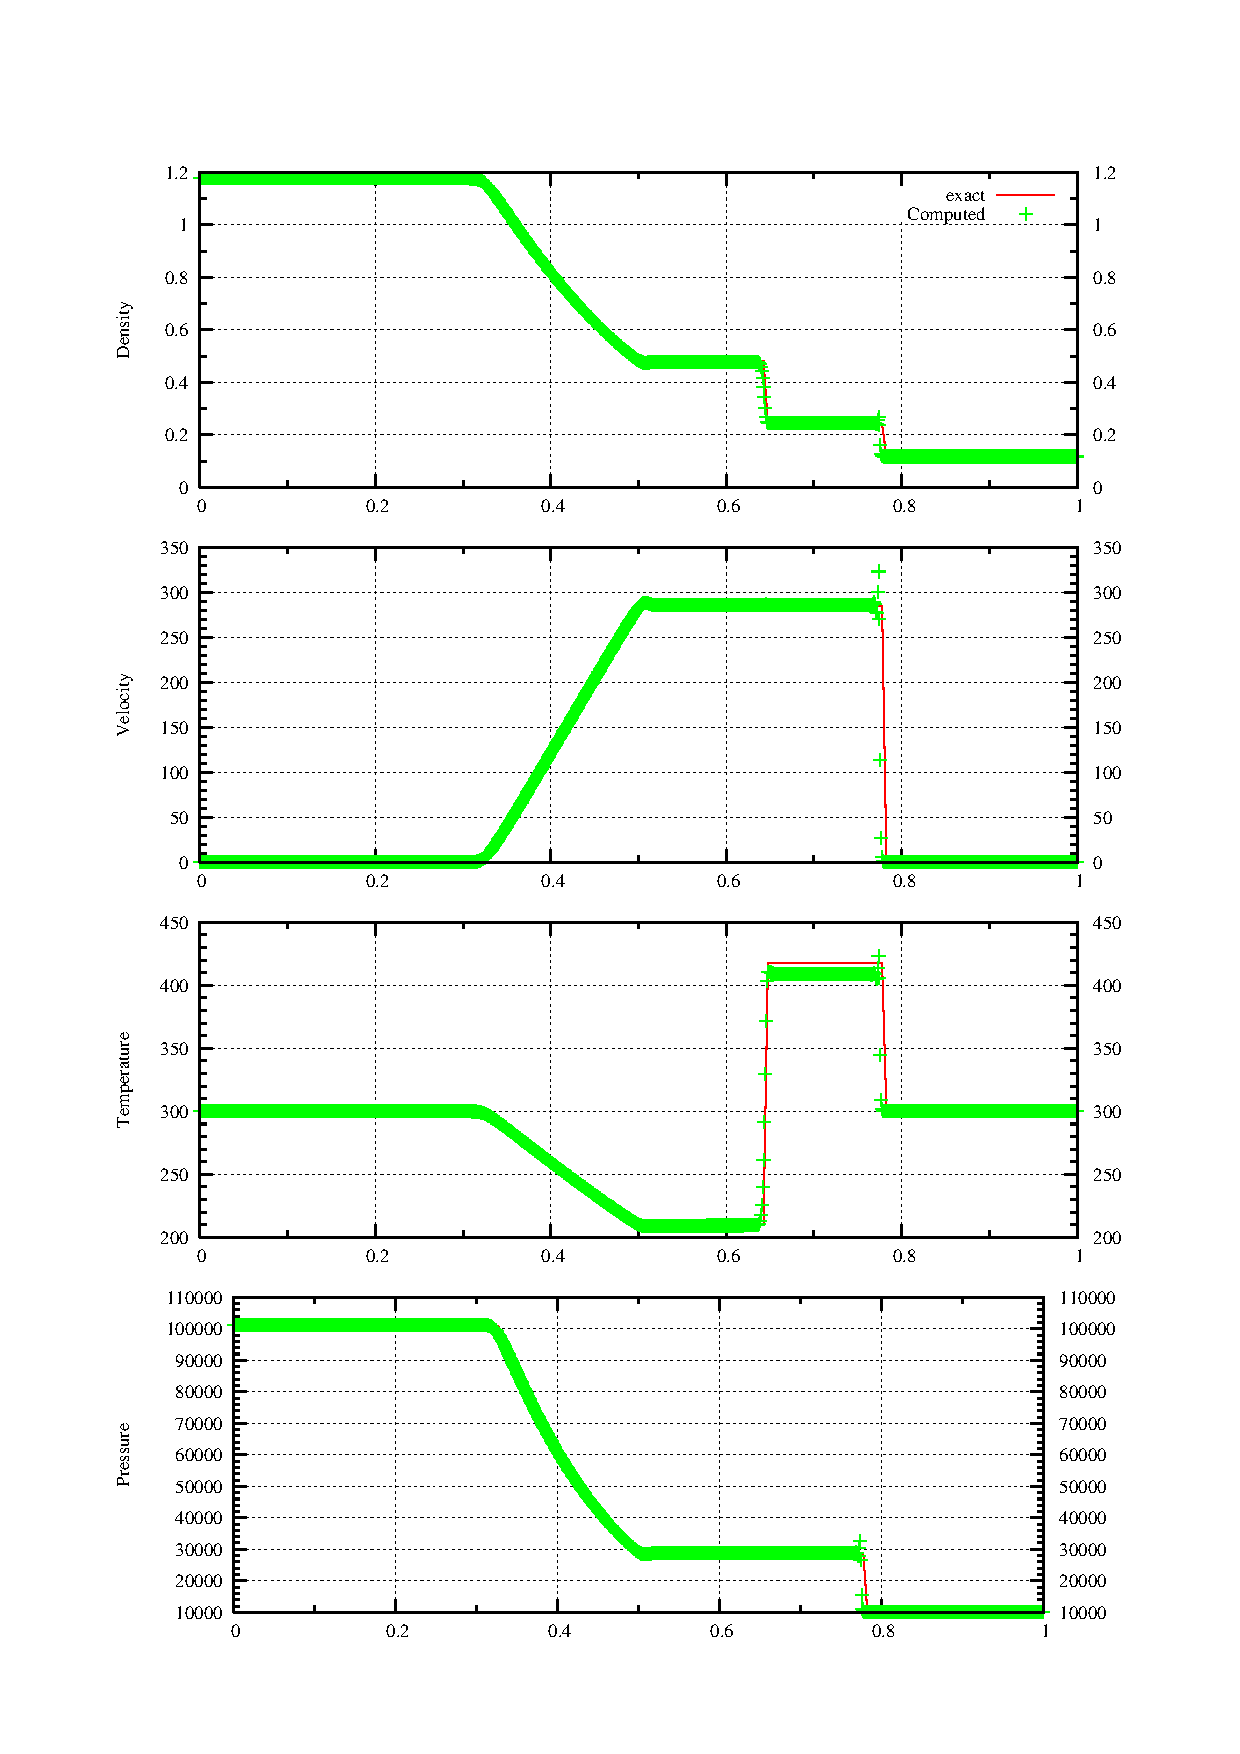
\includegraphics[scale=.65]{shockTube.png}
  \caption{Shock tube results at time $t = 5msec$}
  \label{results.ST}
  \end{figure}
\newpage
%
%__________________________________SHOCKTUBE AMR
\section*{\center Shock Tube with Adaptive Mesh Refinement}
 
\subsection*{\underline{Simulation Specifics}}
\begin{description} 
\footnotesize
\item [Component used:] \hfill ICE
\item [Input file name:] \hfill shocktube\_AMR.ups
\item [Command used to run input file:]\hfill sus inputs/UintahRelease/ICE/shocktube\_AMR.ups
\item [Postprocessing command:]\hfill \\
inputs/UintahRelease/ICE/plot\_shockTube\_AMR shockTube\_AMR.uda y\\
This will generate a postscript file shockTube\_AMR.ps

\item [Simulation Domain:]\hfill    1 x .001 x .001 m
\item [Cell Spacing:] \hfill\\
10 x 1 x 1 mm (Level 0)\\
2.5 x 1 x1 mm (Level 1)\\
0.625 x1 x1 mm (Level 2)

\item [Example Runtimes:] \hfill \\
 2ish minutes   (1 processor, 2.66 GHz Xeon)

\item [Physical time simulated:] \hfill 0.005 sec.

\end{description}

\section*{\underline{Results}}
Figure \ref{results.ST.AMR} shows a comparison of the exact versus simulated results at time $t = 5msec$.
\begin{figure}
  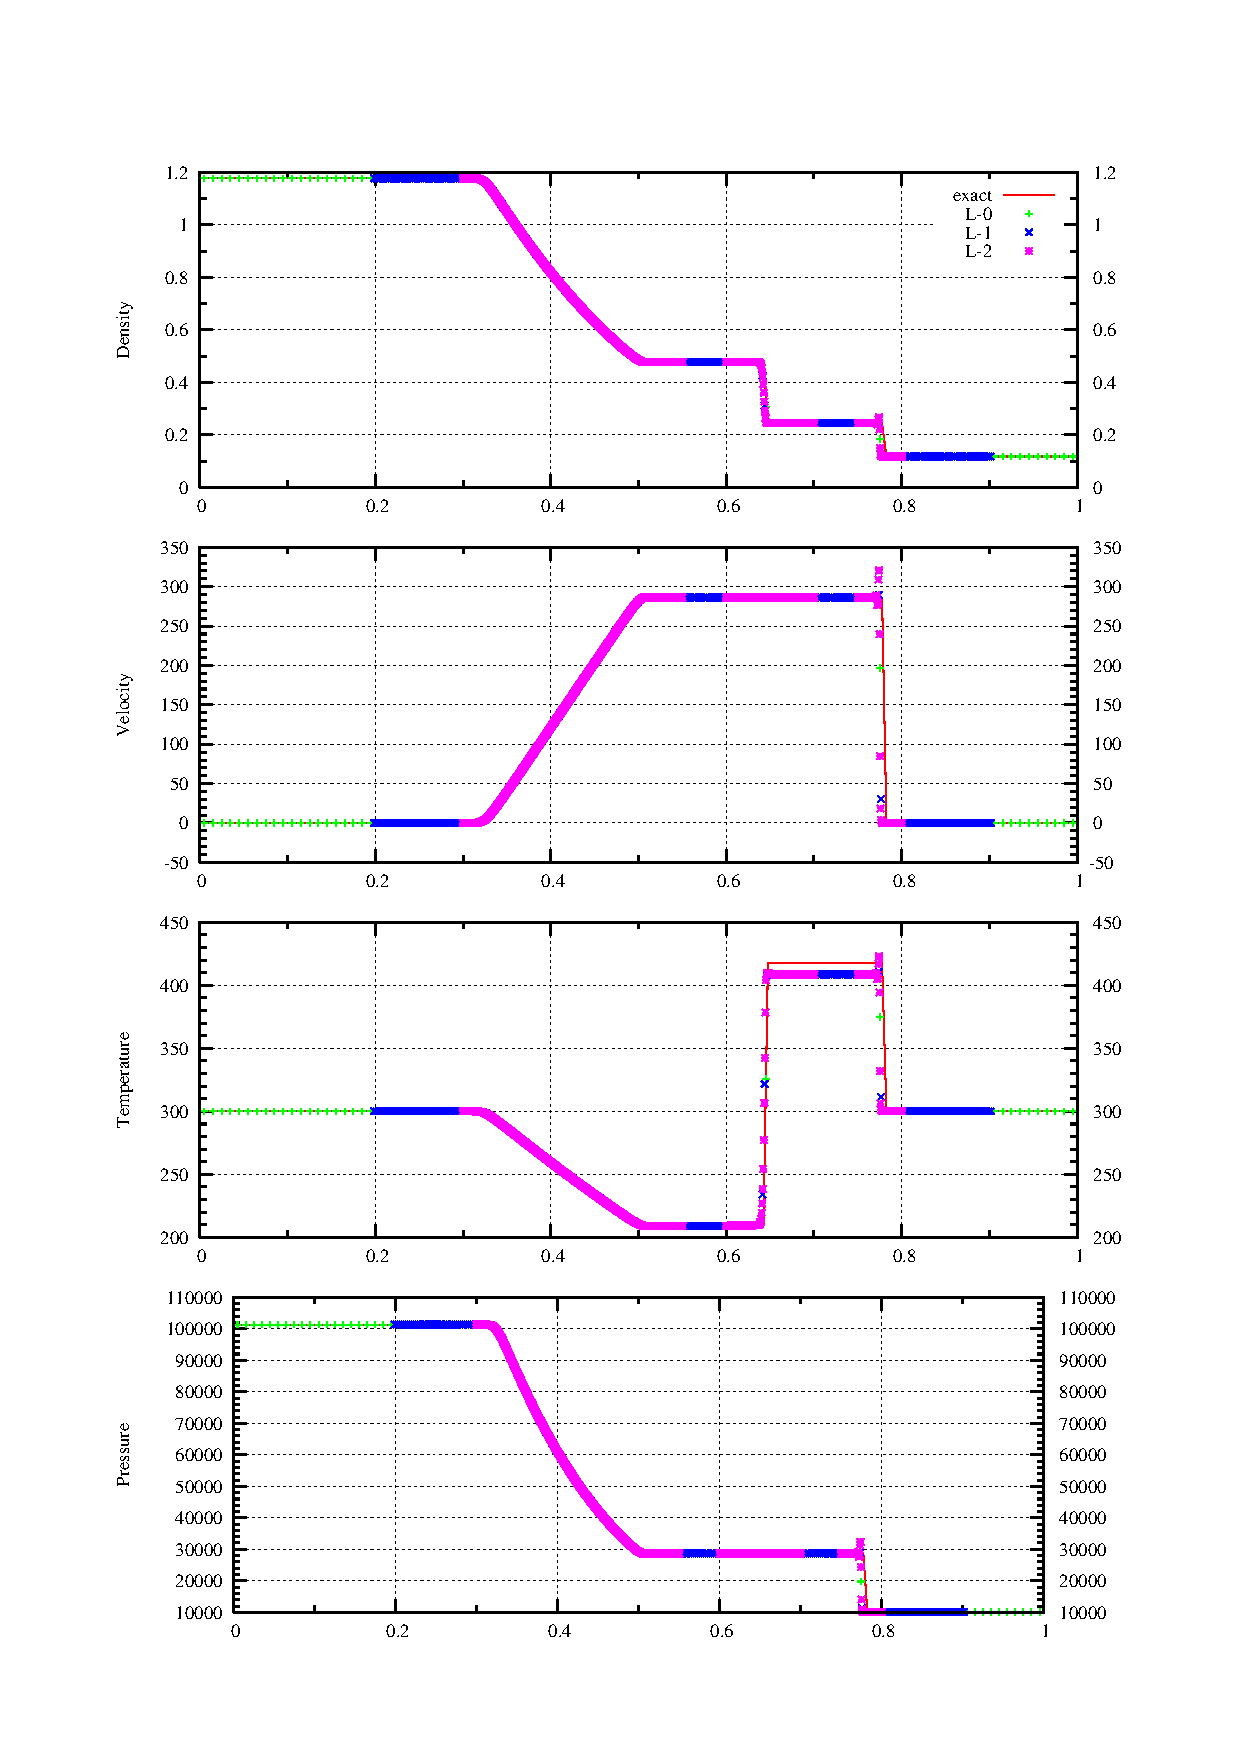
\includegraphics[scale=.85]{shockTube_AMR.png}
  \caption{Shock tube results at time $t = 5msec$}
  \label{results.ST.AMR}
  \end{figure}
\newpage
%
%__________________________________riemann2D
\section*{\center 2D Riemann Problem with Adaptive Mesh Refinement}
\subsection*{\underline{Problem Description}}
In two-dimensional Riemann problems there 15 different solutions that combine
rarefaction waves, shock waves and a slip line or contact discontinuities
\cite{ref:schulz_collins_glaz, ref:Liska_Wendroff}.  Here we simulate 4 slip
lines that form a symmetrical single vortex turning counter clockwise. At
time $t=0$ the computational domain is divided into four quadrants by the
lines $x = 1/2, y=1/2$  The initial condition for $V=(p, \rho, u, v)$ in the
four quadrants are $V_{ll}=(1, 1, -0.75, 0.5), V_{lr}=(1, 3, -0.75,-0.5),
V_{ul}=(1,2,0.75,0.5), V_{ur}=(1,1,0.75,-0.5)$ where, $p$ is pressure,
$\rho$ is the density of the polytropic gas, $u$ and $v$ are the $x$ and $y$
component of velocity.
\subsection*{\underline{Simulation Specifics}}
\begin{description} 
\footnotesize
\item [Component used:] \hfill ICE
\item [Input file name:] \hfill riemann2D\_AMR.ups
\item [Command used to run input file:]\hfill \\
mpirun -np 5 sus inputs/UintahRelease/ICE/riemann2D\_AMR.ups
\item [VisIT session file:]\hfill inputs/UintahRelease/ICE/riemann2D.session
\item [Simulation Domain:]\hfill    0.96 x 0.96m x 0.1 m
\item [Cell Spacing:]\hfill \\ 
40  x 40  x 1 mm (Level 0)\\
10  x 10  x 1 mm (Level 1)\\
2.5 x 2.5 x 1 mm (Level 2)

\item [Example Runtimes:] \hfill \\
 5ish minutes   (5 processors, 2.66 GHz Xeon)
\item [Physical time simulated:] \hfill 0.3 sec.
\end{description}

\section*{\underline{Results}}
Figure \ref{fig:riemann2D} shows a flood and line contour plot(s) of the density of the gas at 0.03sec.
\begin{figure}
  \includegraphics[scale=.6]{riemann2D.png}
  \caption{Contour plot of density for the 2D Riemann problem at time $t = 0.3sec$.  Bottom plot shows the outline of the patches on the 3 levels.}
  \label{fig:riemann2D}
  \end{figure}
\newpage

%__________________________________

\section*{\center Explosion 2D}
\subsection*{\underline{Problem Description}}
For the multidimensional blast wave orexplosion test is a standard compressible
flow problem that has been used by many as a validation test case.  At time
$t=0$ there is a circular region of gas at the center of the domain at a
relatively high pressure and density.  The expansion of high pressure gas
forms a circular shock wave and contact surface that expands into surrounding
atmosphere.  At the same time a circular rarefaction travels towards the
origin.  As the shock wave and contact surface move outwards they become
weaker and at some point the contact reverses direction and travels inward.
The rarefraction reflects from the center and forms an overexpanded region,
creating a shock that travels inward \cite{ref:toro}.  At time $t=0$ the
computational domain is divided into two region, circular high pressure region
with a radius $R=0.4$ and the surrounding box 2x2x0.1.  The initial condition
inside of the circular region were $(p=1, \rho=1, u=0, v=0)$  and outside
$(p=0.1, \rho=0.125, u=0, v=0).$  The fluid was an ideal, inviscid, polytropic gas.
%
\subsection*{\underline{Simulation Specifics}}
\begin{description} 
\item [Component used:] \hfill ICE
\item [Input file name:] \hfill Explosion.ups
\item [Command used to run input file:]\hfill \\
      mpirun -np 4 sus inputs/UintahRelease/ICE/Explosion.ups
\item [Visualization net file:]\hfill inputs/UintahRelease/ICE/Explosion.session\\
\item [Postprocessing command:]\hfill \\
inputs/ICE/Scripts/plot\_explosion\_AMR Explosion\_AMR.uda y\\
This will generate a postscript file explosion\_AMR.ps


\item [Simulation Domain:]\hfill    2 x 2 x .1
\item [Cell Spacing:]\hfill \\ 
62.5    x 62.5    x 10 (Level 0)\\
15.625  x 15.625  x 10 (Level 1)\\
3.9     x 3.9     x 10 (Level 2)

\item [Example Runtimes:] \hfill \\
 20 minutes   (4 processor, 2.66 GHz Xeon)

\item [Physical time simulated:] \hfill 0.25 (non-dimensional).

\end{description}

\section*{\underline{Results}}
Figures \ref{fig:pressExplode,fig:rhoExplode} shows surface plots of the pressure and density at $t=0.25.$  
\newpage
\begin{figure}
  \includegraphics[scale=.5]{explode_press.png}
  \caption{Pressure field at $t=0.25$}
  \label{fig:pressExplode}
\end{figure}
%
\newpage
\begin{figure}
  \includegraphics[scale=.5]{explode_rho.png}
  \caption{Density field at time $t=0.25$}
  \label{fig:rhoExplode}
\end{figure}
\newpage

Since this test is symetrical we can use results from the equivalent 1 dimensional problem to compare against

\begin{figure}
  \includegraphics[scale=.75]{explode_1D.png}
  \caption{XXX$t=0.25$}
  \label{fig:1dExplode}
\end{figure}

\newpage


%__________________________________CH4 fire

%\section*{\center Methane Flame}
%\subsection*{\underline{Problem Description}}
%At $t=0$ Methane gas begin flowing from a $1m$ hole in the floor of the
%computational domain at a velocity of $1m/s$.  The methane mixes with the
%surrounding air, ignites and forms a puffing fire.  The main assumptions in
%this simulation are a) that the chemical reactions are taking place infinitely
%fast (equilibrium chemistry model) and b) that there is no radiative heat
%loss from the product gases.
%\subsection*{\underline{Simulation Specifics}}
%\begin{description} 
%\item [Component used:] \hfill ICE
%\item [Input file name:] \hfill CH4\_fire.ups
%\item [Command used to run input file:]\hfill sus CH4\_fire.ups \\
%Note you must have a link to the {\tt inputs} directory in the save directory as sus.  A table needed
%by the combustion model is inside the {\tt inputs} directory.
%\item [SCIRun visualization net file:]\hfill 3DFire\_Vol.srn \\
%
%
%\item [Simulation Domain:]\hfill    5 x 5 x 5 m
%\item [Cell Spacing:]\hfill \\ 
%3.3 x 3.3 x 3.3 cm (Level 0)
%
%
%\item [Example Runtimes:] \hfill \\
% 8 hours   (64 processor, 2.66 GHz Xeon)
%
%\item [Physical time simulated:] \hfill 3.4sec.
%
%\end{description}
%
%\section*{\underline{Results}}
%Figure \ref{results.CH4} shows a 3D view of the initial puff just before it leaves the computational
%doman.  
%\begin{figure}
%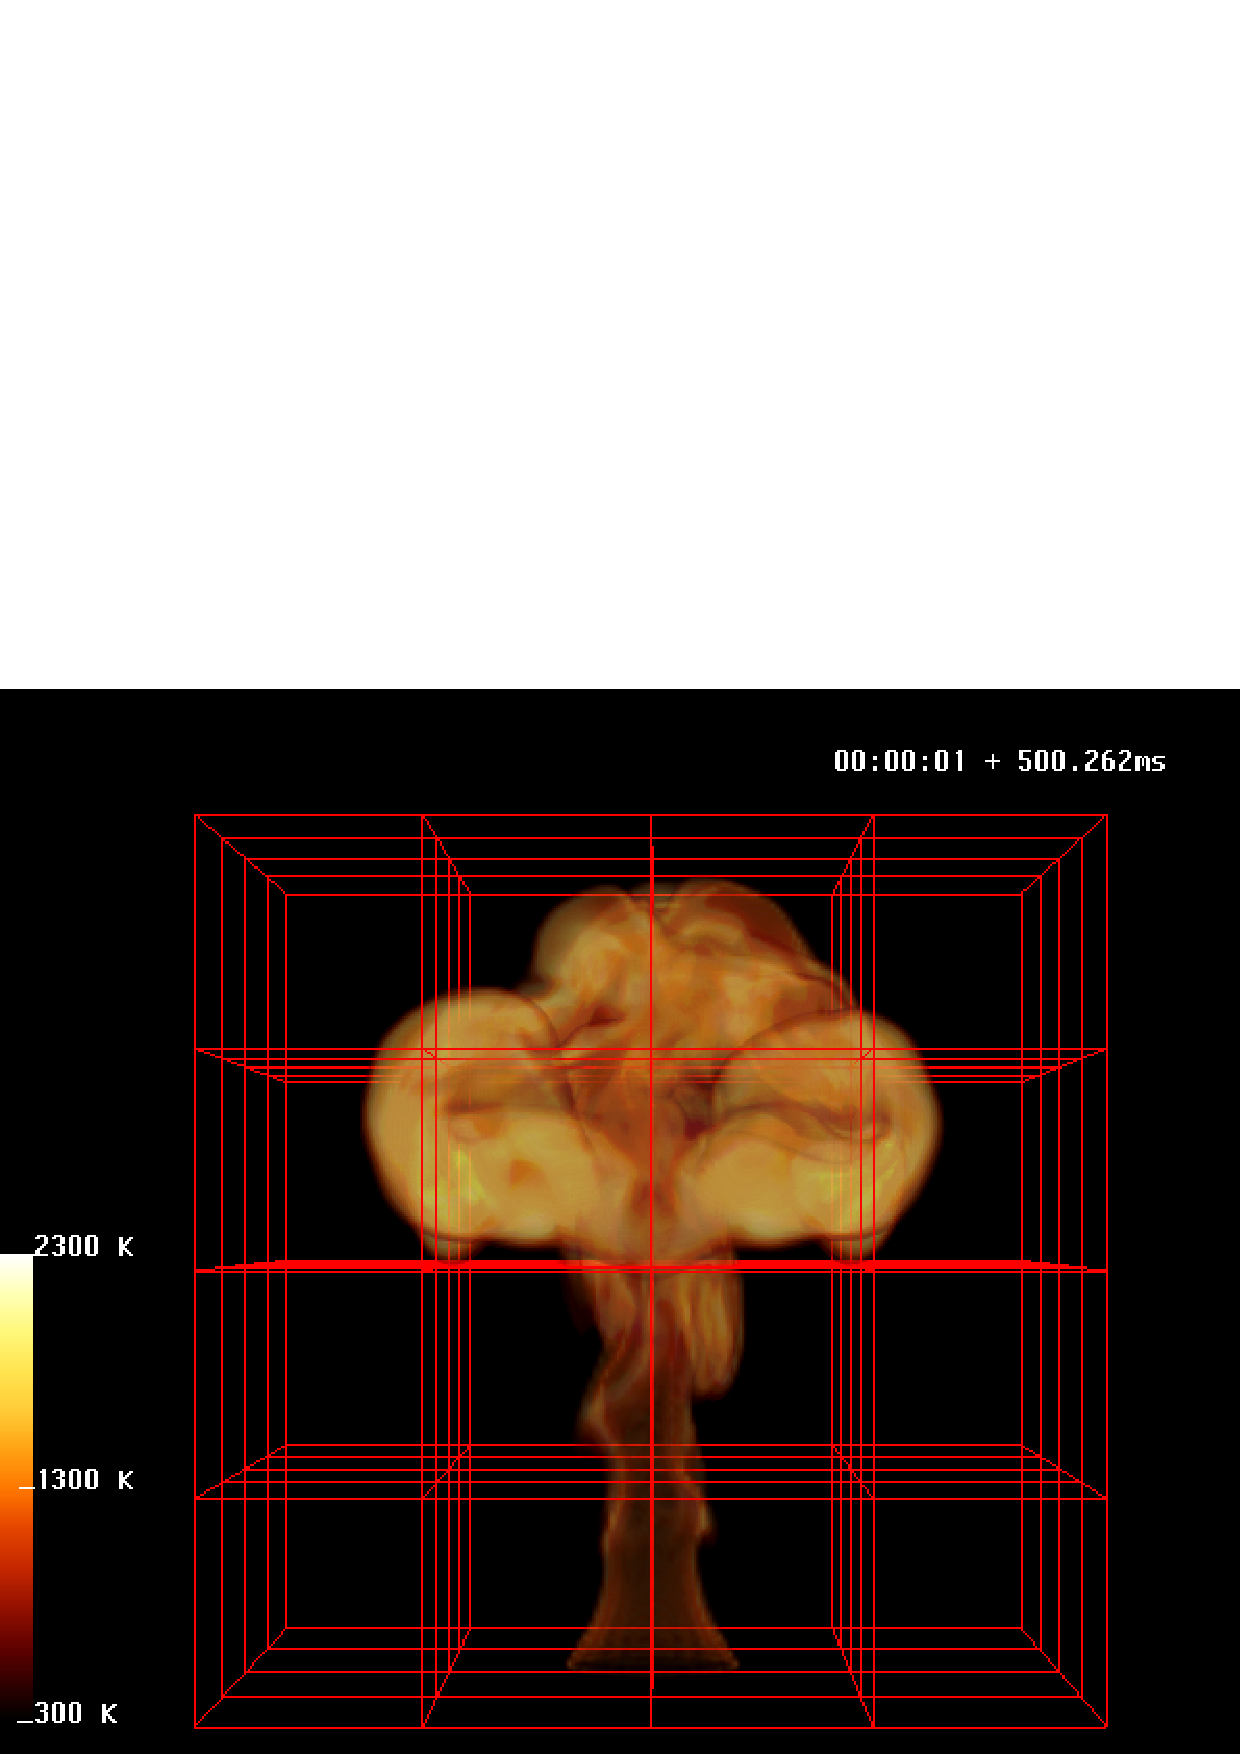
\includegraphics[scale=.66]{3DFire.png}
%\caption{Temperature field at time $t = 1.5 sec$}
%\label{results.CH4}
%\end{figure}
%\newpage


\subsection{References}
\bibliographystyle{plain}
\bibliography{ice}




\section{MPM}

\subsection{Introduction}

\subsection{Theory - Algorithm Description}

\subsection{Uintah Specification}

\subsubsection{Basic Inputs}
\subsubsection{Physical Constants}
\subsubsection{Material Properties}
\subsubsection{Constitutive Models}
\subsubsection{Contact}
\subsubsection{BoundaryConditions}
\subsubsection{Physical Boundary Conditions}

\subsection{Examples}

\subsection{References}

%
\section{MPMArches}

\subsection{Introduction}

\subsection{Theory - Algorithm Description}

\subsection{Uintah Specification}

\subsubsection{Arches}

\subsubsection{Basic Inputs}
\subsubsection{Turbulence}
\subsubsection{Properties}
\subsubsection{BoundaryConditions}
\subsubsection{Physical Constants}
\subsubsection{Solvers}


\subsubsection{MPM}

\subsubsection{Basic Inputs}
\subsubsection{Physical Constants}
\subsubsection{Material Properties}
\subsubsection{Constitutive Models}
\subsubsection{Contact}
\subsubsection{BoundaryConditions}
\subsubsection{Physical Boundary Conditions}

\subsection{Examples}

\subsection{References}


\section{MPMICE} \label{Sec:MPMICE}

\subsection{Introduction}

\subsection{Theory - Algorithm Description}

\subsection{Uintah Specification}

\subsubsection{ICE}

%\subsubsection{Basic Inputs}
%\subsubsection{Physical Constants}
%\subsubsection{Material Properties}
%\subsubsection{Equation of State}
%\subsubsection{Exchange Properties}
%\subsubsection{BoundaryConditions}
%\subsubsection{Solvers}


\subsection{MPM}

%\subsubsection{Basic Inputs}
%\subsubsection{Physical Constants}
%\subsubsection{Material Properties}
%\subsubsection{Constitutive Models}
%\subsubsection{Contact}
%\subsubsection{BoundaryConditions}
%\subsubsection{Physical Boundary Conditions}

\subsection{Examples}

\section*{\center Mach 2 Wedge}
\subsection*{\underline{Problem Description}}
This is a simulation of a symmetric $20^o$ wedge traveling through initially
quiescent air at Mach 2.0.  A shock forms at the leading edge of the
wedge and an expansion fan over its top.  Consultation of oblique shock
tables, e.g.~\cite{Saad} (pp.308-309) reveals that the angle of the leading
shock compares quite well with the expected value.  In addition, this
simulation demonstrates a few other useful features of the fluid-structure
interaction capability.  In this case, the structure is rigid, and as
such, essentially provides a boundary condition to the compressible flow
calculation.  Furthermore, the geometry of the wedge is described via a
triangulated surface, rather than the geometric primitives usually used.
This allows the user to study flow around arbitrarily complex objects,
without the difficulty of generating a body fitted mesh around that object.

\subsection*{\underline{Simulation Specifics}}
\begin{description}
\item [Component used:] \hfill rmpmice (Rigid MPM-ICE)
\item [Input file name:] \hfill Mach2Wedge.ups
\item [Command used to run input file:]\hfill sus Mach2Wedge.ups
(Note: The files wedge40.pts and wedge40.tri must also be copied to
the same directory as sus.)

\item [Simulation Domain:]\hfill    0.25 x 0.0375 x 0.001 m

\item [Cell Spacing:]\hfill \\
.0005 x .0005 x .001 m (Level 0)

\item [Example Runtimes:] \hfill \\
 ~1.5 hours   (1 processor, 3.0 GHz Xeon)\\

\item [Physical time simulated:] \hfill 0.64 milliseconds

\item [Associated visit session:] \hfill Mach2wedge.session

\end{description}

\section*{\underline{Results}}

Figure~\ref{figwedge} shows a snapshot of the simulation.  Contour
plot depicts pressure and reflects the presence of a leading shock
and an expansion fan.
\begin{figure}[b]
  \center
%  \scalebox{0.2}{\includegraphics{Mach2Wedge.png}}
  \caption{$20^o$ wedge moving at Mach 2.0 through initially stationary
air.  Contour plot depicts pressure.}
  \label{figdisks}
\end{figure}

\subsection{References}

\chapter{Glossary} \label{Sec:Glossary}

\begin{itemize}

\item Data Warehouse (NewDW, OldDW, DW) - The \tt Data Warehouse
         \normalfont is an abstraction (and implementation vehicle) used in
         Uintah to provide data to simulation components (across
         distributed memory spaces as necessary).  OldDW refers to a
         DW from the previous time step.  NewDW refers to the DW for
         the current time step.  In practice, variables are usually
         pulled from the OldDW, updated, and placed in the NewDW.

\item Time step - Uintah is a time dependent code.  A time step refers
         to a unique point in simulation time.  The state of the
         simulation is updated one time step at a time.
         
\item Adaptive Mesh Refinement (AMR) - In brief, AMR allows spending
  less CPU time on ``inactive'' (less interesting) areas of the
  simulation, and spend more time computing where there are many
  particles reacting.  Resolution is low in the center where things
  are stable, but high at the edges.  This feature is in ICE, but not
  ARCHES.

\item CCA - Common Component Architecture.

\item CFD - Computational Fluid Dynamics modeling.

\item DistCC - Parallel, distributed compiler.

\item Doxygen - Doxygen (code documentation) web interface.

\item GhostCells (and Extra Cells)

\item Grid - The problem's physical domain.  The number of cells in the
  grid determine the resolution of the simulation.

\item Handle - Smart pointers.  Handles track the number of references
  to a given object, and when the number reaches zero, de-allocates
  the memory.

\item Level - Not a 'level' in 3d-space, but a level of recursion into an
  AMR grid.  ARCHES doesn't support AMR or nonuniform cells, and
  therefore doesn't need recursion, so it works on a single level '1'.

\item Material Point Method (MPM) - The main component for simulating
  structures (physcial objects) in the UCF.

\item Message Passing Interface (MPI) - Communication library used by many
  distributed software packages to communicate data between multiple
  processors.  Besides send'ing and recv'ing data, data
  reduction (UCF Reduction Variables) is supported. 
  \begin{itemize}
    \item OpenMPI
  \end{itemize}

\item Patch - A physical region of the grid assigned one to each
  processor.  The processor working on a patch will compute properties
  for each of the cells contained in the patch.  Think of this as a big
  cube that contains hundreds of little cubes.

\item Regression Tester (RT) - Runs nightly accuracy, memory, and
  completion tests on Uintah simulations.

%\item <table border=''1'' cellpadding=''5'' width=''80%''><tr><td
%                                %bgcolor=''#eeeeff''><b>Programmers
%                                %Note:</b> Programming examples and
%                                %notes will appear like
%                                %this.</td></tr></table>

\item SCIRun - A Problem Solving Environment (PSE) originally used to
  provide core software building blocks for Uintah as well as an
  extensive visualization package for viewing Uintah data archives.

\item SUS - Standalone Uintah Simulator.  This is the main executable
  program in the Uintah project.

\item SVN - Subversion code versioning system.

\item Uintah - The general name of the C-SAFE simulation code.
  Sometimes also refered to as the UCF.  The name comes from the
  Uintah mountain range in Utah.

\item Uintah Computational Framework (UCF) - The core software
  infrastructure for Uintah.
  \begin{itemize}
    \item Variables (CC, NC, FC) - Cell centered, Node centered, and
      Face centered (respectively) data structures used within the UCF.
  \end{itemize}

\item Uintah Data Archive (UDA) - The directory/file/data layout for
  storing Uintah simulation data.

\item Uintah Problem Specification (UPS (Section~\ref{Sec:UPS})) - An XML based file used to
  specify Uintah simulation properties.

\item Uintah Software Organization
  \begin{itemize}
    \item Visualization
    \item scinew - a wrapper for the C++ new() function that allows for memory tracking.
  \end{itemize}

\end{itemize}


% Appendicies
\newpage
% \section*{Appendicies}
% \subsection*{Appendix A. Bomb Units} \label{appendixBombUnits}
\appendix
\addappheadtotoc

\chapter{Bomb Units} \label{appendixBombUnits}

Following is a table of conversion factors from bomb units to mks units.  Bomb units are useful in small scale
simulations that occur very quickly, such as detonation and deformation. \\

\begin{tabular}{|c|c|}
\hline 
\bf{Measure} & \bf{Conversion Factor}     \\
\hline
mass	& $\mu g$               \\
length  & cm                    \\
time    & $\mu s$               \\ [1ex]
kinematic viscosity & $1\frac{\displaystyle cm^2}{\displaystyle \mu s} = 10^2 \frac{\displaystyle m^2}{\displaystyle s}$                          \\ [1ex]
velocity            & $1\frac{\displaystyle cm}{\displaystyle \mu s} = 10^4 \frac{\displaystyle m}{\displaystyle s}$                              \\ [2ex]
force               & $1\frac{\displaystyle \mu gcm}{\displaystyle \mu s^2} = 10 N$                                                               \\ [2ex]
pressure            & $\frac{\displaystyle 10 N}{\displaystyle cm^2} = 10^5 Pa$                                                                   \\ [1ex]
viscosity           & $10^5 Pa \mu s = 10^{-1} Pa s$                                                                                              \\ [1ex]
density             & $1\frac{\displaystyle \mu g}{\displaystyle cm^3} = 1\frac{\displaystyle g}{\displaystyle m^3}$                              \\ [1ex]
heat capacity       & $\frac{\displaystyle 10N cm}{\displaystyle \mu g K} = 10^8 \frac{\displaystyle J}{\displaystyle kg K}$                      \\ [2ex]
power               & $\frac{\displaystyle 10N cm}{\displaystyle \mu s} = 10^5 W$                                                                 \\ [1ex]
thermal conductivity& $\frac{\displaystyle 10^5 W}{\displaystyle cm K} = 10^7 \frac{\displaystyle W}{\displaystyle m K}$                          \\ [2ex]
surface energy      & $\frac{\displaystyle 10 N cm}{\displaystyle cm^2} = 10^3 \frac{\displaystyle J}{\displaystyle m^2}$                         \\ [2ex]
fracture toughness  & $\frac{\displaystyle 10 N}{\displaystyle cm^{\frac{3}{2}}} = 10^{-2} \frac{\displaystyle N}{\displaystyle m^{\frac{3}{2}}}$ \\ [2ex]
enthalpy            & $1\frac{\displaystyle J}{\displaystyle kg} = 10^{-8} \frac{\displaystyle cm^2}{\displaystyle \mu s^2}$                      \\ [2ex]
\hline
\end{tabular}




\end{document} 
